\documentclass[FIPLY_base.tex]{subfiles}

%\author{Gerald Irsiegler}
%\date{26. Februar 2016}

\begin{document}
\section{Übungskatalog}

\subsection{Beschreibung}
Der Übungskatalog beinhaltet eine Liste aller verfügbaren Übungen.

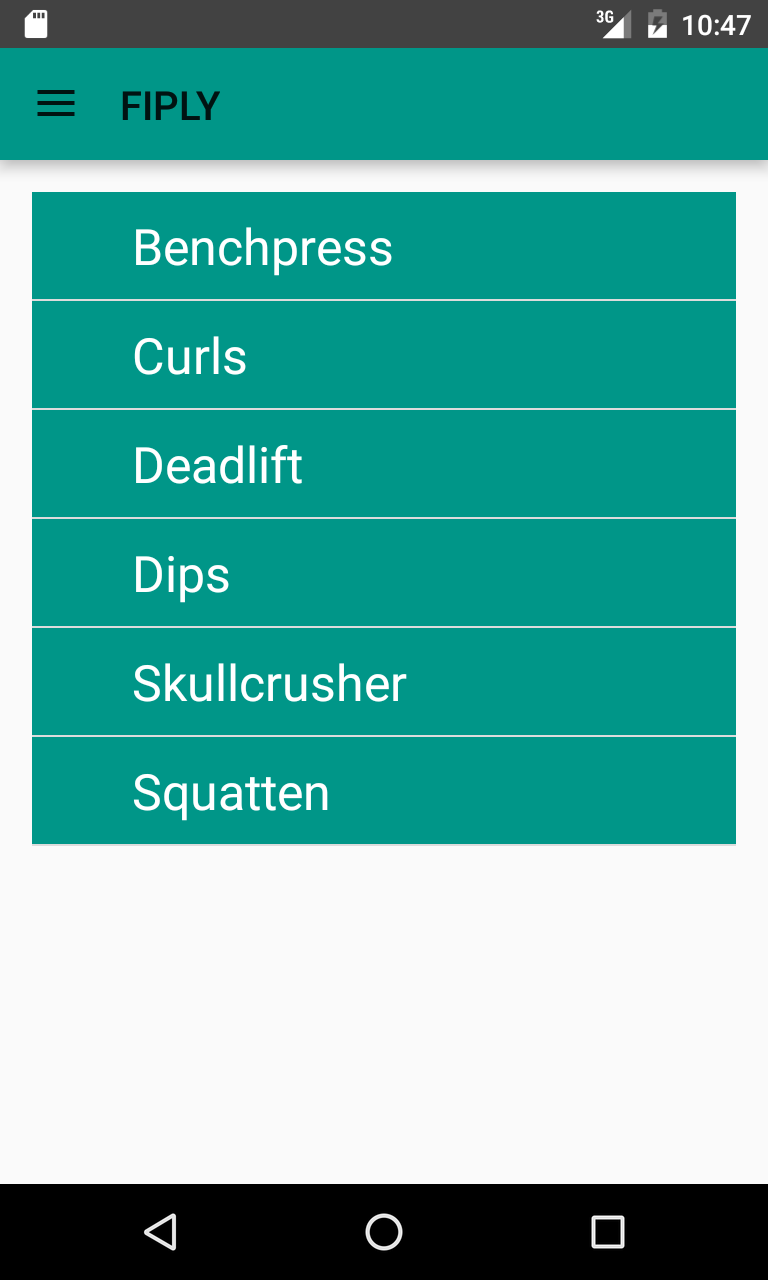
\includegraphics[scale=0.4]{img/Uebungskatalog}

\subsection{Implementierung}
\subsubsection{Expandable List View}
Die Expandable List View ist eine eigene Implementierung der standard List View. Sie erlaubt es bei tippen auf ein Element weitere Unterelemente darzustellen.
Im Laufe der Entwicklung wurde festgestellt, dass eine standard List View, mit einem Verweis auf eine Detail-View vorteilhafter wäre.

\subsubsection{List View}
Die List View zeigt eine Liste aus Element an. Ein Klick auf ein bestimmtes Element löst eine Callback-Methode aus, von welcher die Detail View aufgerufen wird.
\newpage
\subsubsection{Einlesen der Übungen}
Die Informationen über alle Übungen ist in der strings.xml im JSON-Format hinterlegt.
Jede Übung ist somit ihr eigenes JSON-Objekt. 

\begin{lstlisting}
<string name="exercisecatalog">
[
...,
{
  \"Muskelgruppe\":\"Brust,Untere Brust\",
  \"Name\":\"Negativbankdruecken\",
  \"Beschreibung\":\"Mit geradem Ruecken auf Negativbank legen, Wenn ein Polster vorhanden ist - Beine einklemmen, Stange etwa schulterbreit greifen\",
  \"Durchfuehrung\":\"Mit fixierten Schultern die Stange kontrolliert in einer Linie zur Brust und wieder nach oben bewegen, Stange in einer Linie bewegen und Brust nicht beruehren\",
  \"Equipment\":\"Negativbank,Langhantel\",
  \"Schwierigkeit\":\"Mittel\"
}
,...
]
</string>
\end{lstlisting}
Wie in diesem Exampel erkennbar musste jedes Hochkomma mit einem Backslash escaped werden, da der JSON-String sonst nicht in der strings.xml abgelegt werden könnte.
\newpage
\ \\
Dieser JSON-String wird in einer Methode in der UebungenRepository eingelesen und die einzelnen Methoden werden in die Datenbank eingefügt.

\begin{lstlisting}
    public void insertAllExercises() throws JSONException {
        reCreateUebungenTable();
        String json = repoContext.getResources()
                                 .getString(R.string.exercisecatalog);

        JSONArray exercises = new JSONArray(json);
        JSONObject temp;

        for (int i = 0; i < exercises.length(); i++) {
            temp = exercises.getJSONObject(i);
            Log.wtf("Exercise: ", temp.getString("Name"));
            insertUebung(temp.getString("Name"), 
                         temp.getString("Beschreibung"),
                         temp.getString("Durchfuehrung"), 
                         temp.getString("Muskelgruppe"), 
                         temp.getString("Schwierigkeit"), 
                         "https://www.youtube.com/embed/..", 
                         temp.getString("Equipment"));
        }

    }
\end{lstlisting}

\ \\
Diese Methode wird beim Startup der Applikation, während des SplashScreens, in einem Async-Task aufgerufen und ausgeführt.



\newpage


\subsection{DetailView}
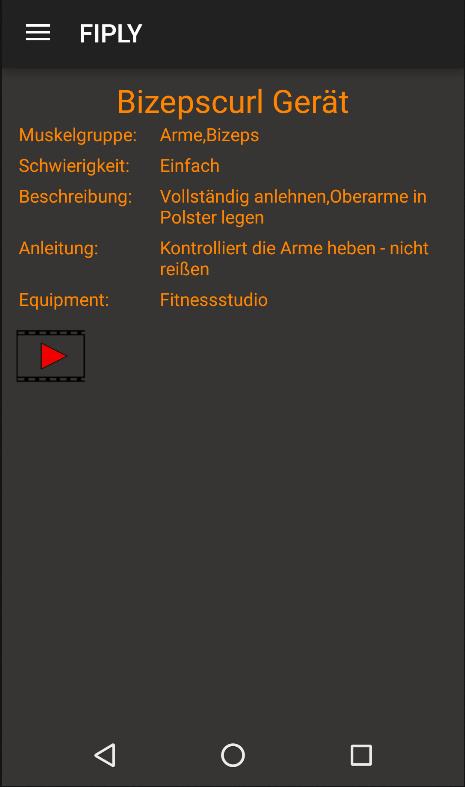
\includegraphics[scale=0.4]{img/Uebungskatalog_detail}


Für jede Übung gibt es eine Detailansicht, in welcher man genaures über jene Übung erfahren kann.
Diese Detail-View wird aufgerufen indem man auf die korrespondierende Übung im Übungskatalog tippt.

Es werden folgende Details bereitgestellt:

\begin{itemize}
\item Name der Übung
\item Die Muskelgruppe/n welche man mit dieser Übung trainiert.
\item Schwierigkeit, wie anspruchsvoll ist diese Übung.
\item Beschreibung, die Ausgangslage der Übung.
\item Anleitung, wie wird die Übung, von der Ausgangsposition, richtig durchgeführt.
\item Benötigtes Equipment, um die richtige Durchführung der Übung zu ermöglichen.
\item Ein Video welches die Durchführung beschreibt. Dieses kann im mit Tipp auf das Videosymbol im linken mittleren Bereich der Detail View aufgerufen werden.
Die App ändert dann automatisch in den Landschafts-Modus und stellt das Video im Vollbildmodus dar.

\end{itemize}



\subsection{Filter}
\subsubsection{Beschreibung}
Die Liste kann auch nach Name der Übung und Muskelgruppe gefiltert werden. 
Der Filter wird über den Floating Action Button aufgerufen, welcher sich in der rechten unteren Ecke des Übungskataloges befindet.
Die Muskelgruppen-Auswahl erfolgt über das Tippen auf eine bestimmte Muskelgruppe, beim Namen wird rein nach Text filtriert

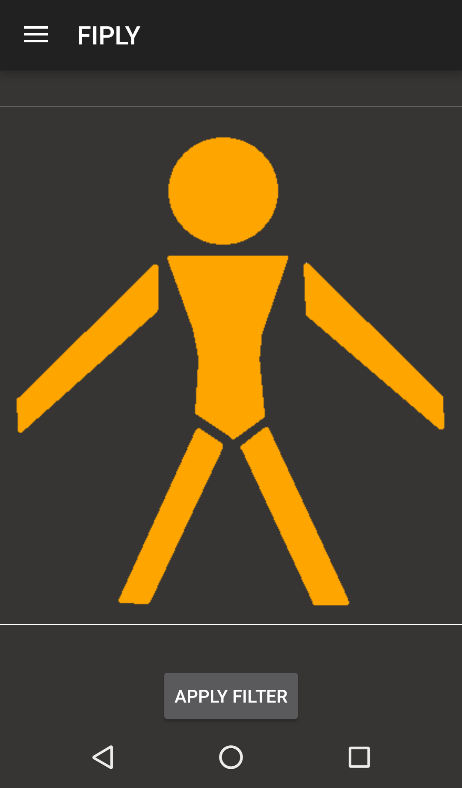
\includegraphics[scale=0.4]{img/Uebungskatalog_filter}
\newpage

\subsubsection{Implementierung}
Für den Filter für Name und Muskelgruppe gibt es jeweils einen Eintrag in der Key-Value-Repository.
Beim Einlesen der Uebungen werden die Filter automatisch angewandt.

\ \\
Die folgende Lösung wurde diesem Tutorial entnommen  [\citetitle{ueClickableAreas} \cite{ueClickableAreas}]

\ \\
Um die geklickte Muskelgruppe zu ermitteln, wurden zwei Auswahlbereiche übereinander gelegt.

\ \\
Jener Auswahlbereich, welchen der Benutzer zu sehen bekommt.
Dieser Auswahlbereich ist nur die visuelle Stütze für den Benutzer, sie hat keinerlei funktionalen Nutzen.

\ \\

\includegraphics[scale=0.4]{img/Uebungskatalog_filter_overlay}

\ \\
Und eine farbkodierte Maske, welche der Benutzer nicht sieht, mit welcher er aber eigentlich interagiert.
Bei einem Klick auf die Auswahlfäche kann nachvollzogen werden welche Farbe der angeklickte Bereich hat, somit wird festgestellt welche Muskelgruppe der Benutzer ausgewählt hat.

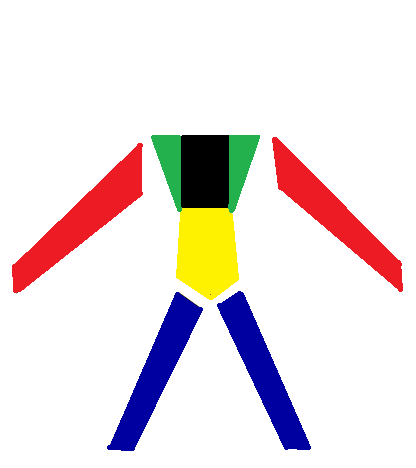
\includegraphics[scale=0.4]{img/Uebungskatalog_filter_mask}

\newpage
\ \\
Bei einem Klick auf die Auswahlfläche wird folgende Callback-Methode aufgerufen.
\begin{lstlisting}
public boolean onTouch(View v, MotionEvent event) {
   int tolerance = 25;
   int evX = (int) event.getX();
   int evY = (int) event.getY();
   int clickedColor = getHotspotColor(evX, evY);

   //RED area is arms
   if (closeMatch(getResources().getInteger(R.integer.redInt), clickedColor, tolerance)) {
      Log.wtf("Area clicked: ", "Arme");
      kvr.updateKeyValue("filterMuskelGruppe", "Arme");
   }
   //BLACK area is Breast
   else if (closeMatch(getResources().getInteger(R.integer.blackInt), clickedColor, tolerance)) {
      Log.wtf("Area clicked: ", "Brust");
      kvr.updateKeyValue("filterMuskelGruppe", "Brust");
   }
   //GREEN area is shoulders
   else if (closeMatch(getResources().getInteger(R.integer.greenInt), clickedColor, tolerance)) {
      Log.wtf("Area clicked: ", "Schultern");
      kvr.updateKeyValue("filterMuskelGruppe", "Schultern");
   }
   //BLUE are is legs
   else if (closeMatch(getResources().getInteger(R.integer.blueInt), clickedColor, tolerance)) {
      Log.wtf("Area clicked: ", "Beine");
      kvr.updateKeyValue("filterMuskelGruppe", "Beine");
   }
   //YELLOW area is core(stomach)
   else if (closeMatch(getResources().getInteger(R.integer.yellowInt), clickedColor, tolerance)) {
      Log.wtf("Area clicked: ", "Bauch");
      kvr.updateKeyValue("filterMuskelGruppe", "Bauch");
   }
   return true;
}
\end{lstlisting}
Diese Methode ermittelt die Farbe des gedrückten Bereiches und setzt den Key-Value Eintrag im Repository.
\newpage
\ \\
Die erste verwendete Hilfsmethode ermittelt ob zwei Farbwerte ähnlich oder gleich sind.

\begin{lstlisting}
    public boolean closeMatch(int color1, int color2, int tolerance) {
        if (Math.abs(Color.red(color1) - Color.red(color2)) > tolerance)
            return false;
        if (Math.abs(Color.green(color1) - Color.green(color2)) > tolerance)
            return false;
        if (Math.abs(Color.blue(color1) - Color.blue(color2)) > tolerance)
            return false;
        return true;
    }
\end{lstlisting}

\ \\
Die zweite verwendete Methode ermittelt den Farbwert des gedrückten Bereichs.
\begin{lstlisting}
    public int getHotspotColor(int x, int y) {
        bodyFilterMask.setDrawingCacheEnabled(true);
        Bitmap hotspots = Bitmap.createBitmap(bodyFilterMask.getDrawingCache());
        bodyFilterMask.setDrawingCacheEnabled(false);
        return hotspots.getPixel(x, y);
    }
\end{lstlisting}


\end{document}
